\documentclass{article}

% Language setting
% Replace `english' with e.g. `spanish' to change the document language
\usepackage[english]{babel}

% Set page size and margins
% Replace `letterpaper' with `a4paper' for UK/EU standard size
\usepackage[letterpaper,top=1cm,bottom=2cm,left=2cm,right=2cm,marginparwidth=1.75cm]{geometry}
\usepackage[utf8]{inputenc}
\usepackage[T1]{fontenc}
\usepackage[english]{babel}
\usepackage{ifpdf,amsmath,amsthm,amssymb,amsfonts,newtxtext,newtxmath} 
\usepackage{array,graphicx,dcolumn,multirow,hanging}
\usepackage[labelfont=sc,textfont=sf]{caption}
\usepackage[hyperfootnotes=false,breaklinks=true]{hyperref}
\urlstyle{rm}
\usepackage[hyphenbreaks]{breakurl}

% Useful packages
\usepackage{amsmath}
\usepackage{graphicx}
%\usepackage[colorlinks=true]{hyperref}
\usepackage[colorlinks=true, allcolors=blue]{hyperref}
%%%%%
\usepackage{tikz}
\usetikzlibrary{shapes.geometric, arrows}
\usepackage{pbox}
\usepackage{lipsum}
%%%%%
\newcommand\totalrandomized{1088}
\newcommand\pmales{75.3 \%}
\newcommand\meanage{41.0}
\newcommand\meandropout{35.4 \%}
\newcommand\ptseeking{79.9 \%}
\newcommand\ppsyd{75.2\%}
\newcommand\psudd{10.9 \%}
%%%%%%%



\title{Ondansetron in alcohol use disorder: a systematic review}
\author{}
\date{}

\begin{document}
\maketitle

\begin{abstract}
\textbf{Context} Alcohol use disorder (AUD) is a frequent disorder. Few treatments have shown a great efficacy in clinical studies. It is hypothetized that this is due to the fact that AUD suffering people constitute a heterogeneous group composed of various endophenotypes. Ondansetron, a selective $\text{5-HT}_3$ receptor antagonist, has been evaluated in AUD and partciularly in certain subgroups of patients. This review presents clinical studies evaluating its impact.\\ 
\textbf{Methods} A systematic review was conducted on Pubmed and Wiley Online Library. All 19 clinical trials involving the use of ondansetron in AUD where included.\\
\textbf{Results} Ondansetron was found to be effective mostly in certain subgroups of AUD-suffering patients. The identified subgroups were based on clinical evaluation (age of onset, personality type) and genotype. A number of limitations remains and further studies are needed.\\
\textbf{Keywords} \textit{alcohol use disorder, ondansetron, $\text{5-HT}_3$ receptors, serotonin, craving, pharmacogenetics, personnalized medicine}
\end{abstract}

\section*{Introduction}
\paragraph{}
Alcohol use disorder (AUD) is a heterogeneous and chronic relapsing disorder resulting in a complex interaction between neurobiological, genetic and environmental factors. Despite the demonstrated efficacy of some approved medications (acamprosate, naltrexone, disulfiram), a key barrier is the fact that these medications are not effective in every patient pointing out the need for more personalized therapy approaches to overcome this heterogeneity. In this perspective, major advances in pharmacogenetics have highlighted distinct clinical subgroups of AUD according to genetic variation, that could be associated with differential treatment responses. Thus, the identification of patient subtypes that are most likely to respond favorably to different medications is crucial with a need for a better targeting of medication to specific patients.

\paragraph{}
Amongst the emerging pharmacotherapies for AUD, Ondansetron (IUPAC name: (RS)-9-Methyl-3- [(2-methyl-1H-imidazol1-yl)methyl]-2,3-dihydro-1Hcarbazol-4(9H)-one), a selective antagonist of the $\text{5-HT}_3$ receptor, has shown some promising results. Ondansetron is approved by ANSM in France and FDA in the USA as an antiemetic for cancer treatment-induced and anesthesia related nausea and vomiting. 
In the late 1980s, Hagan et al. \cite{hagan_effect_1987} showed that the injection of ondansetron in the ventral tegmental area of the rat brain lessened induced hyperactivation in the nucleus accumbens, pointing out the tight relationship between serotonin function and the mesolimbic dopaminergic reward system. Based on these findings and the role of dopaminergic activity on the rewarding effects of alcohol, ondansetron was thought to attenuate the pleasurable subjective effects of alcohol and thereby to reduce alcohol consumption in AUD suffering patients. Some phase 1 clinical studies (\cite{grant_blockade_1991}, \cite{johnson_attenuation_1993}) found promising results in healthy male volunteers, and provided preliminary evidence on the role of ondansetron in reducing the reinforcing properties of alcohol and the desire to use by 5-HT3 receptor blockade. 
Later phase 2 clinical studies (\cite{johnson_ondansetron_2000}, \cite{kranzler_effects_2003}) suggested differential effects among AUD patients depending on the age of onset (Early-onset alcoholism EOA/Late-onset alcoholism LOA) \cite{varma1994correlates}, which is hypothesized to be linked to individual genetic variations. Interestingly, compared to placebo, ondansetron was associated with reduced drinking and significant reduction in overall craving in randomized placebo-controlled studies (\cite{johnson_ondansetron_2000}, \cite{johnson_ondansetron_2002}), but only among patients who developed AUD before age 25 only (EOA), and not among late-onset patients (LOA), presumably by ameliorating serotonergic abnormality.

\paragraph{}Furthermore, as the functional state of the serotonin transporter protein (5-HTT) is an important factor of the serotonergic function control, more recent pharmacogenetic studies have investigated the potential role of 5-HTT genotype on drinking behaviors and alcohol craving ([7]). 5-HTT gene polymorphisms, involving two variants, a short form (S) and a long form (L), have been shown to be associated with differential 5-HT neurotransmission, which could moderate the rewarding effects and the craving for alcohol, and thereby ondansetron treatment response among AUD suffering patients. In line with this hypothesis, ondansetron was administered in a large study among AUD patients according to the 5-HTT polymorphism (ref Johnson 2011). Participants with the LL genotype significantly reduced their drinking compared to the LS or SS genotype, suggesting that ondansetron could represent an interesting approach for the personalized treatment of AUD according to specific polymorphism of the 5-HTT gene.

\paragraph{}Direct inhibition of the 5-HT3 receptor is thus hypothesized to reduce alcohol use and alleviate alcohol craving, that is currently considered as a key determinant of relapse vulnerability as well as a major treatment target. A better knowledge of the potential impact of 5-HT antagonist medication on alcohol consumption and craving in AUD, as well as individual clinical subtypes and genotype associated with treatment response is therefore a critical issue to improve treatment approaches and develop personalized medicine in the pharmacotherapy of alcohol use disorder. The aim of this systematic review is to address this issue by assessing scientific evidence of the efficacy of ondansetron on alcohol consumption and craving as well as clinical or genetic predictors of treatment response.

%-------------------------------------------------------------------------------------------------------------------------------------------------------------------
\section*{Methods}
\paragraph{Research design}
The study involved a systematic review of the literature based on the Preferred Reporting Items for Systematic reviews and Meta-Analyses (PRISMA) guidelines \cite{page2021prisma}.

\paragraph{Databases and search strategy}
This review was based on the following databases: PUBMED/MEDLINE, Psychinfo, Cochrane, Wiley Online Library. The search was performed for all years up to December, 2021. 

The following search terms were used:

For Medline search, the relevant articles were identified by combining the terms: ("ondansetron"[MeSH Terms] OR "ondansetron"[All Fields]) AND ("alcoholism"[MeSH Terms] OR "alcoholism"[All Fields] OR "alcohol use disorder"[All Fields] OR "alcohol abuse"[All Fields] OR "AUD"[All Fields])

For the Wiley Online Library search we used the keywords "ondansetron" AND "alcoholism".

For the PsycInfo search, the keywords were "ondansetron or Zofran" AND "alcoholism or alcohol dependence or alcohol abuse or alcoholic or alcohol addiction".

Finally, the Cochrane Library was used by searching ("alcohol use disorder" OR "alcohol dependance") AND "ondansetron" in "Title Abstract Keyword".

\paragraph{Eligibility criteria}
Studies were included if they met the following inclusion criteria :
\begin{itemize}
 \item Reported as a peer reviewed journal
    \item Concerning individuals suffering from AUD, with no restrictive criteria regarding age, sex, ethnic origin, or place of living.
    \item Assessing the impact of ondansetron on AUD and/or predictors of ondansetron treatment response.
    \item Papers published in English.
\end{itemize}

Studies were excluded if: 
\begin{itemize}
    \item Reviews, opinion papers, protocols, case reports,
    \item Preclinical studies
    \item Studies in healthy volunteers
    \item Not published in English
\end{itemize}

\paragraph{Study selection}
Two authors independently examined all titles and abstracts. Relevant articles were obtained in full-text and assessed for inclusion criteria separately by the two reviewers based on the inclusion and exclusion criteria previously mentioned. Disagreements were resolved via discussion of each article for which conformity to inclusion and exclusion criteria were uncertain and a consensus was reached. The reference lists of major papers were also manually screened in order to ensure comprehensiveness of the review. All selected studies were read in full to confirm inclusion criteria, study type and study population.

\paragraph{Assessment of risk of bias in included studies} 
Two review authors independently assessed the risk of bias of each included study using the revised Cochrane tool for assessing risk of bias in randomised trials (RoB 2 \cite{sterne2019rob}), in accordance with methods recommended by Cochrane collaboration. The risk-of-bias plot in Figure~\ref{fig:trafficlight} was generated using the Robvis online tool \cite{mcguinness_risk--bias_2021}. The following judgements were used : high risk, low risk or unclear (either lack of information or uncertainty over the potential for bias). Authors resolved disagreements by consensus, and a third author was consulted to resolve disagreements if necessary.

The Newcastle Ottawa Scale (NOS, \cite{peterson2011newcastle}) was used for assessing single-arm non randomized studies. However, it had to be adapted by removing the Comparability item for two of the studies that lacked a control group.

\paragraph{Data collection}
Sample characteristics (including socio-demographic data, age, gender, comorbidity), information on study design, eligibility criteria and exclusion criteria, study duration and location, clinical outcome assessment methods, dropout rate and treatment dosage were extracted.
%-------------------------------------------------------------------------------------------------------------------------------------------------------------------------------------------
\section*{Results} 

%\input{tables/table}
%%%%%%%%%%%%%%%%%%%%%%%%%%%%%%%%%%%%%%%%%%%%%%%%

\paragraph{Study selection}
A total of 90 results were found in the MEDLINE database, 68 on PsycInfo, 35 on Cochrane Library and 8 additional studies were found on Wiley Online Library.  

A total of 134 articles were identified through the search of the databases. After review of titles, 40 articles were selected for further examination.

After reading the full text, 21 met inclusion criteria for this review. This process is described in the PRISMA flowchart (Figure~\ref{fig:flowchart}). 

Among the 21 included studies, 18 were randomized controlled trials (RCT) or analysis of previous RCT, and 3 were prospective open-label studies (\cite{kranzler_effects_2003}, \cite{dawes_prospective_2005}, \cite{dawes_reductions_2005}). The study duration ranged from 2 to 12 weeks. The selected articles were published between 1994 and 2015. 

\paragraph{Quality assessment and risk of bias}
Randomized controlled trials where analyzed using the Cochrane Rob2 tool (see Figure~\ref{fig:trafficlight} for the traffic-light plot). Two studies had a low concern of bias (\cite{sellers_clinical_1994}, \cite{myrick_effect_2008}), most of the studies showed some concern of bias and one had a high concern (\cite{correa_filho_pilot_2013}).
The high dropout rate of the studies was the most concerning factor and affected the Domain 3 of the Risk of Bias tool which represent bias due to missing outcome result.
For the 3 prospective study, the Newcastle-Ottawa scale was used (see Figure~\ref{tab:nos}). The risk of bias was evaluated as acceptable as one study scored 7 out of 9 possible points and the two others scored 6 out of 7 (adapted score).

\subsubsection*{Study results}
Results are presented according to their primary outcomes. Among the 21 included studies, 17 directly assessed ondansetron efficacy through alcohol use (n=12), craving (n=5) and mood effect (n=2). Four studies examined moderators of treatment outcomes.
The first set of studies (Tables~\ref{tab:e1}, \ref{tab:e2}, \ref{tab:e3}) investigated alcohol use, craving and mood disturbances as clinical outcomes for ondansetron efficacy, while the second set (Table~\ref{tab:m}) examined the moderators of treatment outcomes. 
%%%%%%%%%%%%%%%%%%%%%%%%%%%%%%%%%%%%%%%%
\paragraph{Sample characteristics}

The included studies involved 11 distinct study populations whom characteristics are described in Table~\ref{tab:pop}.

In total, \totalrandomized\ subjects were enrolled, of which 1071 (98.4\%) met criteria for alcohol use disorder. Patients were mostly males (n=819; \pmales\%), with a mean age of \meanage.

Patients enrolled were diagnosed as alcohol dependent according to the DSM-III-TR (\cite{sellers_clinical_1994}, \cite{johnson_ondansetron_2000}), DSM-IV (\cite{myrick_effect_2008}, \cite{johnson_combining_2000}, \cite{ait-daoud_combining_2001}, \cite{kranzler_effects_2003}, \cite{dawes_prospective_2005}, \cite{johnson_pharmacogenetic_2011}), DSM-IV-TR (\cite{kenna_within-group_2009}, \cite{kenna_ondansetron_2014-1}), DSM-5 (\cite{sherwood_brown_randomized_2021}) or ICD-10 (\cite{correa_filho_pilot_2013}).
Some studies required additional criteria, such as more than 35 standard drinks per week for men or 28 for women (\cite{kenna_within-group_2009}, \cite{kenna_ondansetron_2014-1}), more than 30 drinks per week for men or 21 for women (\cite{seneviratne_serotonin_2012}), at least 15 standard drinks in the week before enrollement (\cite{sherwood_brown_randomized_2021}), more than 3 standard drinks per day and a Michigan Alcohol Screening Test greater than 5 (\cite{johnson_combining_2000}, \cite{johnson_ondansetron_2000}, \cite{ait-daoud_combining_2001}), an AUDIT score greater than 8 (\cite{johnson_pharmacogenetic_2011}) or a diagnose before the age of 25 (\cite{sherwood_brown_randomized_2021}).
Whereas most trials (\cite{sellers_clinical_1994}, \cite{johnson_combining_2000}, \cite{johnson_ondansetron_2000}, \cite{ait-daoud_combining_2001}, \cite{kranzler_effects_2003}, \cite{dawes_prospective_2005}) concerned treatment-seeking patients, some (\cite{myrick_effect_2008}, \cite{kenna_within-group_2009}, \cite{kenna_ondansetron_2014-1}) did not. With the exclusion of nicotine and alcohol, drug use and disorder was considered as an exclusion criteria in most included studies. Thus, participants who reported drug use (\cite{kranzler_effects_2003}, \cite{myrick_effect_2008}, \cite{kenna_within-group_2009}, \cite{johnson_pharmacogenetic_2011}, \cite{kenna_ondansetron_2014-1}) and/or had a positive drug screening test (\cite{sellers_clinical_1994}, \cite{johnson_combining_2000}, \cite{johnson_ondansetron_2000}, \cite{ait-daoud_combining_2001}, \cite{myrick_effect_2008}, \cite{correa_filho_pilot_2013}]) were often excluded, except for cannabis use in a few trials (\cite{dawes_prospective_2005}, \cite{myrick_effect_2008}). Receipt of alcohol use disorder treatment prior to enrollment was an exclusion criteria; one study (\cite{sellers_clinical_1994}) considered treatment over the previous 12 months, and 3 (\cite{johnson_age_2000}, \cite{ait-daoud_combining_2001}, \cite{dawes_prospective_2005}) over the previous 30 days. 

Some studies excluded participants who had been treated with stimulants, sedatives, hypnotics or with treatment that could have an effect on alcohol consumption or mood (\cite{correa_filho_pilot_2013}, \cite{johnson_ondansetron_2000}, \cite{johnson_combining_2000}, \cite{ait-daoud_combining_2001}, \cite{dawes_prospective_2005}). In one study (\cite{sherwood_brown_randomized_2021}), having been treated with naltrexone, acamprosate, disulfiram or topiramate 2 weeks prior inclusion, or current treatment with phenytoin, carbamazepine, rifampicine, apomorphine or tramodol (due to potential interactions with ondansetron) were exclusion criteria.

Psychiatric disorders were exclusion criteria in most studies (\cite{johnson_ondansetron_2000}, \cite{johnson_combining_2000}, \cite{ait-daoud_combining_2001} \cite{kranzler_effects_2003}, \cite{kenna_within-group_2009}, \cite{johnson_pharmacogenetic_2011}, \cite{kenna_ondansetron_2014}). Two studies considered only major diagnosis (\cite{myrick_effect_2008}) or clinically significant disorders (\cite{correa_filho_pilot_2013} \cite{dawes_prospective_2005}) as exclusion criteria. In the study of Sellers et al. (\cite{sellers_clinical_1994}), a Montgomery/asberg Depression scale score below 15 and a Spielberger State-Trait anxiety inventory score below 55 were required. In contrast, one study (\cite{sherwood_brown_randomized_2021}) enrolled only people with a concurrent psychiatric diagnosis.

Many studies also required good health at enrollment and notably excluded frequent AUD comorbidities such as elevated bilirubin (\cite{johnson_ondansetron_2000}, \cite{kenna_within-group_2009}), liver enzymes (\cite{dawes_prospective_2005}, \cite{kenna_within-group_2009}, \cite{sherwood_brown_randomized_2021}), liver cirrhosis (\cite{correa_filho_pilot_2013}, \cite{sherwood_brown_randomized_2021}) or severe alcohol withdrawal (\cite{johnson_combining_2000}, \cite{johnson_ondansetron_2000}, \cite{dawes_prospective_2005}, \cite{sherwood_brown_randomized_2021}).

%%%%%%%%
Considering participants subtypes, 9 studies (\cite{johnson_ondansetron_2000}, \cite{johnson_combining_2000}, \cite{ait-daoud_combining_2001}, \cite{ait-daoud_combining_2001-1}, \cite{johnson_ondansetron_2002}, \cite{johnson_ondansetron_2003}, \cite{kranzler_effects_2003}, \cite{roache_prediction_2008}), \cite{sherwood_brown_randomized_2021}) focused on clinical characteristics based on age of onset, before or after the age of 25 (EOA and LOA, while 6 studies examined patient subtypes according to their genotypes (\cite{johnson_pharmacogenetic_2011}, \cite{seneviratne_serotonin_2012}, \cite{johnson_determination_2013}, \cite{kenna_ondansetron_2014}, \cite{kenna_ondansetron_2014-1}, \cite{hou_subgroup_2015}). The most frequent investigated gene was SLC6A4, coding for the serotonin transporter that contains a polymorphism in the promoter region, the 5-HTT-linked polymorphic region, with a "short" (S) and "long" (L). Other genes of interest were HTR3A and HTR3B, which regulate the 5HT3 receptor had polymorphisms which influenced response to ondansetron (rs1150226-AG and rs1176713-GG in HTR3A and rs17614942-AC in HTR3B).

Ondansetron dosage was between 1 µg/kg bid (twice a day) and 16 mg per day with the most frequent dosage being 4 µg/kg bid. One study (\cite{sherwood_brown_randomized_2021}) used a flexible dosage which varied in function of treatment response and could range from 0.5 to 4 mg bid (with mean dose at exit being 3.24 ± 2.64 mg/day). Four studies (\cite{johnson_combining_2000}, \cite{ait-daoud_combining_2001}, \cite{ait-daoud_combining_2001-1}, \cite{myrick_effect_2008}) involving 127 patients in total used ondansetron in combination with naltrexone at a dosage of 50 mg per day. Three studies (97 patients) evaluated ondansetron against sertraline, at a dosage of  200 mg per day (\cite{kenna_within-group_2009}, \cite{kenna_ondansetron_2014}, \cite{kenna_ondansetron_2014-1}).
Treatment duration ranged from 8 days to 11 weeks. Pill count or riboflavin dosage were used for assessing treatment compliance

%%%%%%%%%%%%%%%%%%%%%%%%%%%%%%%%%%%%
%ICI !!! = page 6 du word

%%%%%%%%%%%%%%%%%%%%%%%%%%%%%%%%%%%%
\paragraph{Treatment outcomes} 
Efficacy was most often assessed by evaluating the number of standard drinks and derived variables such as defined by the Alcohol Timeline Followback (TLFB) method \cite{sobell1996timeline}. Drinking outcomes were drinks per day (DD), drinks per drinking day (DDD), percentage of day abstinent (PDA), heavy drinking days (days with more than 5 drinks per day) percentage of heavy drinking day (PHDD). Standard drink definition varied between different studies, it was defined as 12 g (\cite{johnson_ondansetron_2000}\cite{johnson_pharmacogenetic_2011}), 13 g (\cite{sellers_clinical_1994} or 14 g\cite{correa_filho_pilot_2013}) of pure ethanol.

Some studies (\cite{ait-daoud_combining_2001}, \cite{johnson_ondansetron_2002}\cite{myrick_effect_2008}) evaluated alcohol craving, either with a visual analogical scale or with the obsessive compulsive drinking scale (OCDS \cite{anton1996obsessive}). One study (\cite{dawes_reductions_2005}) used the Adolescent Obsessive–Compulsive Drinking Scale (A-OCDS) and another (\cite{sherwood_brown_randomized_2021}) the Penn Alcohol Craving Scale (PACS) to assess craving.

One study (\cite{myrick_effect_2008}) used functional magnetic resonance imaging to determine ventral striatum activation. Another study used the Profile of Mood States \cite{mcnair1989profile} to evaluate attenuation of mood disturbances.
Finally, one study (\cite{sherwood_brown_randomized_2021}) used Hamilton Rating Scale for Depression (HRSD), Young Mania Rating Scale (YMRS), and Inventory of Depressive Symptomatology–Self-report (IDS-SR).

A few studies measured carbohydrate deficient transferrin (CDT) (\cite{johnson_ondansetron_2000}, \cite{ait-daoud_combining_2001-1}, \cite{kranzler_effects_2003}, \cite{sherwood_brown_randomized_2021}) as an objective measure of alcohol use. Three studies (\cite{kenna_within-group_2009}, \cite{kenna_ondansetron_2014}, \cite{kenna_ondansetron_2014-1}) measured  or the volume of alcohol consumed in an alcohol self administration. $\gamma$-glutamyltransferase levels were used as an outcome in one study (\cite{sherwood_brown_randomized_2021}).
%variables/instruments for alcohol use and craving measures (cliniques/imagerie) 

%Impact of ondansetron on alcohol use and alcohol craving 
%%%%%%%%%%%%%%%%%%%%%%%%%%%%%%%%%%%%%

%%%%%%%%%%%%%%%%%%%%%%%%%%%%%%%%%%%%%%%%%%%%%%%%%%%%%%%%%%%%%%%%%%%%%%%%%%%%%%%%%%%%%%%%%%%%%%%%%%%%%%%%%%%%%%%%%%%%%%%%%%%%%%%%%%%%%%%

\paragraph{Study results}
The 21 clinical trials where subdivided in two main subgroups according to their primary outcomes. The first set of studies (Tables \ref{tab:e1}, \ref{tab:e2} and \ref{tab:e3}) evaluated the efficacy of ondansetron, by evaluating its impact on alcohol use, craving and mood disturbances. The second set (Table \ref{tab:m}) evaluated the moderators of treatment outcomes.
%%%%%%%%%%%%%%%%%%%%%%%%%%%%%%%%%%%%%%%%%%%%%%%%%%%%%%%%%%%%%%%%%%%%%%%%%%%%%%%%%%%%%%%%%%%%%%%%%%%%%%%%%%%%%%%%%%%%%%%%%%%%%%%%%%%%%%%

\paragraph{Alcohol use reduction}
Eleven studies, summarized in Table~\ref{tab:e1} evaluated the impact of ondansetron, alone or in combination with naltrexone on alcohol use. The main outcomes were mostly self-reported changes in alcohol consumption in standard drinks (using the previously defined TLFB method). A few studies used objective measures: plasma CDT (\cite{johnson_ondansetron_2000}, \cite{ait-daoud_combining_2001-1}, \cite{kranzler_effects_2003}, \cite{sherwood_brown_randomized_2021}), GGT (\cite{sherwood_brown_randomized_2021}) or the volume of alcohol consumed in an alcohol self administration  (\cite{kenna_within-group_2009}, \cite{kenna_ondansetron_2014}, \cite{kenna_ondansetron_2014-1}).

In a sample of 71 males suffering from alcohol dependence (DSM-III-TR), Sellers \textit{et al.} \cite{sellers_clinical_1994} showed a trend (p = 0,06), and \textit{post hoc} analysis indicated a significative impact on AUD patients drinking less than 10 drinks a day. The effect of ondansetron was shown to be non-linear, as 0,25 mg was more effective than 2 mg.

In a small scale randomized control trial \cite{johnson_combining_2000} (n = 20, exclusively EOA), a combination of ondansetron and naltrexone showed significant effect on reduction of drinks per day (0.99 $\pm$ 0.60 vs 3.68 $\pm$ 0.63, effect size = 1.42) and drinks per drinking day (3.14 $\pm$ 0.87 vs 6.76 $\pm$ 0.71, effect size = 1.71), as well as a trend in reducing the percentage of abstinent days, compared to placebo.

A subsequent analysis of the sample by Ait-Daoud \textit{et al.} showed that the combination of ondansetron and naltrexone was associated with significantly lower CDT levels \cite{ait-daoud_combining_2001-1}.

In a later trial (Johnson \textit{et al.} 2000b \cite{johnson_ondansetron_2000}), 271 patients of the 321 enrolled were given ondansetron at various dosages (1, 4 and 16 µg/kg of body weight, twice a day). In this study, ondansetron was found to be significantly more effective than placebo in reducing alcohol consumption among EOA but not LOA. Ondansetron at 4 µg/kg \emph{b.i.d.}, which was (non significantly) superior to the other dosages, was more effective than placebo on drinks per day (1.56 vs 3.30, p = 0.01), drinks per drinking day (4.28 vs 6.90, p = 0.004), percentage of day abstinent (70.10 vs 50.20, p = 0.02) and mean log CDT ratio (-0.19 vs 0.12, p = 0.01). Among EOA, all other dosages were superior to placebo on the two first criteria.

These results were subsequently replicated by Kranzler \textit{et al.} in 2003 \cite{kranzler_effects_2003}, who showed a significant reduction (compared to baseline) in most alcohol-related measures (drinks per day, drinks per drinking days, DrinC total score) among EOA and LOA who received ondansetron (4 µg/kg \emph{b.i.d.}. A significant difference was also found between EOA and LOA receiving ondansetron, benefiting the former on drinks per day, drinks per drinking day and DrinC total score. 

A larger-scale clinical trial, conducted by Johnson \textit{et al.} \cite{johnson_pharmacogenetic_2011}, enrolling 283 patients  showed that L/L-subjects receiving ondansetron significantly reduced their alcohol consumption, measured by drinks per drinking day and percentage of days abstinent as compared to placebo (respectively -1.62, p = 0.007 and 11.27\%, p = 0.023).

In a small-scale study with 15 non-treatment seeking individuals, Kenna \textit{et al.} \cite{kenna_within-group_2009} showed that patient with L/L genotype on the 5-HTTPLPR promoter region of SLC6A4 (further referred as L/L-subjects) that were administered ondansetron (4 µg/kg \emph{b.i.d.}) for 3 weeks drank significantly less alcohol at an alcohol self-administration, compared to similar patients administered sertaline (200 mg per day).

Another clinical trial involving 77 patients, showed limited support that ondansetron may reduce drinking in non-treatment seeking L/L-subjects and was inconclusive in evaluated the effectivness of sertraline in S/L or S/S-subjects (\cite{kenna_ondansetron_2014-1}). Further analysis (\cite{kenna_ondansetron_2014}) pinpointed gender differences as L/L women treated with ondansetron and S/L or S/S women treated with sertraline had significantly less drinks per drinking days and drank less at alcohol self-administration evaluations.

In the only trial taking place outside of North America, Corrêa Filho \textit{et al.} \cite{correa_filho_pilot_2013} showed a significative reduction of heavy drinking days (7,8 \% vs 11,7\%, p=0.02) but not of other measured outcomes.

Recently, Sherwood \textit{et al.} \cite{sherwood_brown_randomized_2021} evaluated the efficacy of ondansetron in 70 patients suffering from both amcohol use disorder and bipolar disorder. Results showed a trend in greater reduction of drinking as measured by the TLFB method that failed to reach significance.
%%%%%%%%%%%%%%%%%%%%%%%%%%%%%%%%%%%%%%%%%%%%%%%%%%%%%%%%%%%%%%%%%%%%%%%%%%%%%%%%%%%%%%%%%%%%%%%%%%%%%%%%%%%%%%%%%%%%%%%%%%%%%%%%%%%%%%%

\paragraph{Craving and cue-induced craving}
Four studies (Table~\ref{tab:e2}) evaluated the impact of ondansetron on craving.

An analysis of the study population of Johnson \textit{et al.} 2000a (\cite{johnson_combining_2000}) found that the combination of ondansetron and naltrexone was significantly better than placebo at reducing craving among EOA \cite{ait-daoud_combining_2001}.

Johnson \textit{et al.} 2002 \cite{johnson_ondansetron_2002} showed that ondansetron at 4 µg/kg \emph{b.i.d.} was associated with a significant reduction in craving (measured by visual analog scale) compared to the placebo group, but only in EOA. In contrast, craving was significantly increased by ondansetron at 1 µg/kg \emph{b.i.d.} among LOA.

In a BOLD-MRI laboratory study, Myrick \textit{et al.} \cite{myrick_effect_2008} evaluated ventral striatum activation of AUD suffering people, treated for 7 days by either naltrexone, ondansetron, a combination of both or placebo, and "social-drinkers" (control group), when shown alcohol cues or neutral beverage cues. Ventral striatum activation was significantly reduced in the naltrexone, combination and social-drinkers groups. This was correlated with reduced craving scores in these groups. Ondansetron alone wasn't significantly effective in the reduction of ventral striatum activation nor craving. There was however a trend in the reduction of both.

Sherwood \textit{et al.} \cite{sherwood_brown_randomized_2021} evaluated craving with the PACS but found no differences between ondansetron and placebo groups, among patients with bot bipolar disorder and AUD. 
%%%%%%%%%%%%%%%%%%%%%%%%%%%%%%%%%%%%%%%%%%%%%%%%%%%%%%%%%%%%%%%%%%%%%%%%%%%%%%%%%%%%%%%%%%%%%%%%%%%%%%%%%%%%%%%%%%%%%%%%%%%%%%%%%%%%%%%

\paragraph{Mood disturbances}
One study, presented in Table~\ref{tab:e3}, showed that among EAO only, ondansetron significantly reduced mood disturbances as measured by the POMS scale (\cite{mcnair1989profile}).

Sherwood \textit{et al.} \cite{sherwood_brown_randomized_2021} showed that ondansetron was significantly more efficacious than placebo in the reduction of HRSD scores, but not of YMRS or IDS-SR scores, among patients suffering from both bipolar disorder and AUD.
%%%%%%%%%%%%%%%%%%%%%%%%%%%%%%%%%%%%%%%%%%%%%%%%%%%%%%%%%%%%%%%%%%%%%%%%%%%%%%%%%%%%%%%%%%%%%%%%%%%%%%%%%%%%%%%%%%%%%%%%%%%%%%%%%%%%%%%

\paragraph{Moderators of treatment outcomes}
Finally, six studies, presented in Table~\ref{tab:m} didn't directly evaluate the efficacy of ondansetron but provided useful information on predicton factors or safety and tolerability.

As ondansetron had previously been found useful in early onset alcoholism, Dawes \textit{et al.} \cite{dawes_prospective_2005} evaluated ondansetron among adolescent in a prospective, open-label trial, which showed that ondansetron was safe and well tolerated in adolescents with alcohol dependence. In a subsequent study \cite{dawes_reductions_2005}, they found that reduction of drinking (as assest by TLFB) was correlated with reduction in craving, as measured by POCS.

Roache \textit{et al.} 2008 \cite{roache_prediction_2008} compared the prediction capabilities of the EOA/LOA typology to the type A/type B typology precedently described by Babor \textit{et al.} 1992 \cite{babor1992a}\cite{babor1992b}(derived from Type I/II description by Cloninger \textit{et al.} \cite{cloninger1987systematic}). The A/B typology better described baseline severity of alcohol dependence but treatment response to ondansetron was significantly better predicted by the EOA/LOA typology.

Seneviratne \textit{et al.} \cite{seneviratne_serotonin_2012} produced some evidence that 5'-HTTPLR mRNA levels could be used as biomarker to evaluate treatment effectiveness in L/L-subjects treated with ondansetron.

Two studies analysed the population of Johnson \textit{et al.} 2011 \cite{johnson_pharmacogenetic_2011} and identified genotypes predicting treatment success. Johnson \textit{et al.} 2013 \cite{johnson_determination_2013} found 5 genotypes which presence predicted efficacy of ondansetron and which where present in a third of the population. Finally,  Hou \textit{et al.} \cite{hou_subgroup_2015} further worked on identifying ways of predicting effectivness of ondansetron and found that data mining approaches, such as interaction trees and virtual twins could simplify subgroup identification while limiting statistical errors.
%%%%%%%%%%%%%%%%%%%%%%%%%%%%%%%%%%%%%%%%%%%%%%%%%%%%%%%%%%%%%%%%%%%%%%%%%%%%%%%%%%%%%%%%%%%%%%%%%%%%%%%%%%%%%%%%%%%%%%%%%%%%%%%%%%%%%%%%%%%%%%%%

%-------------------------------------------------------------------------------------------------------------------------------------------------------------------------------------------------------
\section*{Discussion}
To our knowledge, this paper is the only systematic review including every clinical trial involving the use of ondansetron for the treatment of alcohol use disorder. A subsequent research identified 5 systematic reviews in the last 10 years that included the keywords 'ondansetron' and 'alcohol use disorder' or 'alcoholism'. Bauer \textit{et al.} 2015 \cite{bauer_serotonergic_2015} focused on the influence of serotonergic gene variation in substance use pharmacotherapy and included four out of the 21 studies presented here. Naglich \textit{et al.} 2018 \cite{naglich_systematic_2018} focused on combined pharmacotherapy for the treament of alcohol use and thus included 2 studies involving ondansetron and naltrexone. Cservenka \textit{et al.} 2017 \cite{cservenka_review_2017} focused on pharmacogenetics and the implication of ethnic diversity in the treatment of AUD and included 2 papers. Castrén \textit{et al.} 2019 \cite{castren_selecting_2019} focused on the recent findings in AUD pharmacoterapy and mentioned ondansetron without including any of the clinical trials. Finally, Bharadwaj \textit{et al.} 2018 \cite{bharadwaj_pharmacotherapy_2018} focused on the pharmacotherapy for relapse prevention in AUD in the Indian setting and also mentioned ondansetron but didn't include any trial on this topic.

One review \cite{thompson_variation_2016} focuses on the role of the serotonin transporter gene in AUD and thus cites 6 of the latest pharmacogenetics studies.

Most of the clinical trials described in this systematic review have stringent inclusion criteria which greatly limits their external validity. Particularly, patients suffering from dual diagnosis or addicted to several substance (with the exception of nicotine) were often excluded. 

The high dropout rate (mean dropout rate 35.4\%) could impact the validity of the findings, but evidence to identify whether or not dropout rate favors medication is lacking.

Finally, out of the seven registered trials that have no published papers yet, three haven't had any updates for more than ten years whereas one reported non significant results. This may pose a publication bias that is to be taken in consideration.

\paragraph{Conclusion} 

Whereas growing evidence tends to suggest efficacy of ondansetron as a treatment of alcohol use disorder in particular genetic subgroups, nsew studies will be needed to fully conclude. In particular, there is a need for bigger studies evaluating long term changes in alcohol consumption. These studies should also have less exclusion criteria to maximize their external validity.

%%%%%%%%%%%%%%%%%%%%%%%%%%%%%%%%%%%%%%%%%%%%%%%%%%%%%%%%%%%%%%%%%
%10 dernière années :

%- la revue la plus complète contient 4 des articles et évalue son efficacité (mais se concentre plus généralement sur tous les médicaments qui influence la sérotonine) (Bauer 2015)

%- une revue inlcut 2 des articles, et porte sur les combinaison de traitement dans le TUA 'naglich)

%- une revue inclut 2 des articles, mais porte sur les conséquences de l'ethnicité sur la réponse aux traitements (Cservenka 2017)

%- une revue l'aborde mais n'inclut aucune des études (sujet : pharmacothérapie du TUA, sur les 2 dernières années) (Castren 2019)

%- la dernière mentionne l'ondansetron comme potentiellement intéressant mais déclare qu'il n'y a pas d'études disponibles sur le sujet (Bharadwaj 2018).

%%%%%%%%%%%%%%%%%%%%%%%%%%%%%%%%%%%%%%%%%%%%%%%%%%%%%%%%%%%%%%%%%

%une revue non systématique porte sur un sujet très proche, les variations du gène de la sérotonine et le TUA, et mentionne les 6 études de pharmacogénétiques (l'article est écrit par les auteurs de ces études) (Thomson 2016)

\renewcommand{\refname}{\spacedlowsmallcaps{References}} % For modifying the bibliography heading

\bibliographystyle{unsrt}

\bibliography{references.bib} % The file containing the bibliography
%-----------------
\newpage

\begin{table*}[]
  \centering
   \caption{Population description}
  \label{tab:pop}
\begin{tabular}{llllllllll}
 \hline
%------------------------------------------------------------
&&&&&&&&&\\
 &
\pbox{5cm}{Original publication;\\subsequent analysis} & 
\pbox{5cm}{Location} & 
\pbox{5cm}{Sample\\size} & 
\pbox{5cm}{Males\\(\%)} &
\pbox{5cm}{Mean \\age} &
\pbox{5cm}{Dropout\\rate} & \pbox{5cm}{Treatment\\seeking} & 
\pbox{5cm}{Excluded\\PD} & \pbox{5cm}{Other\\SUD$\ddagger$} \\ %
&&&&&&&&&\\
 \hline
%-------- PANDA ----------------------------------------------------
A
& Sellers 1994 \cite{sellers_clinical_1994} 
& Toronto, Canada %Canada, Toronto 
& 86 
& 100 \%
& 43.6% (9.7)
& 17.4 \% %15/86
& \textbf{yes}
& \textbf{no}$\ast$
& no
\\
%---------------------------------------------
B
& Johnson 2000a \cite{johnson_combining_2000}; \cite{ait-daoud_combining_2001}\cite{ait-daoud_combining_2001-1} 
& San Antonio, USA
& 20
& 75 \%
& 38.0% (1.78)
& 30 \% %1 full, 30% not all visits
& \textbf{yes}
& yes
& no
\\
%---------------------------------------------
C
& Johnson 2000b \cite{johnson_ondansetron_2000}; \cite{johnson_ondansetron_2002}\cite{johnson_ondansetron_2003}\cite{roache_prediction_2008} 
& Houston, USA
& 271% randomized, 271 randomized in \cite{johnson_ondansetron_2000}, 253 in \cite{johnson_ondansetron_2002}
& 70 \%
& 40.6% (0.88)
& 42 \% %1-158/271
& \textbf{yes}
& yes
& no
\\
%---------------------------------------------
D
& Kranzler 2003 \cite{kranzler_effects_2003}
& Farmington, USA 
& 40
& 67.5 \%
& 43.7% (9.76)
& 30 \% %1-28/40
& \textbf{yes}
& yes
& no
\\
%---------------------------------------------
E
& Dawes 2005a \cite{dawes_prospective_2005}; \cite{dawes_reductions_2005}
& San Antonio, USA
& 12
& 58.3 \%
& 18% (2.13)%calc
& 25 \%%3/12
& \textbf{yes}
& \textbf{no}$\ast$
& \textbf{yes}$\dagger$
\\
%---------------------------------------------
F
& Myrick 2008 \cite{myrick_effect_2008}
& Northridge, USA
& 107%17 social drinkers, 90 alcohol dependant
& 72.9 \%
& 25.7
& N.A.
& no
& yes
& \textbf{yes}$\dagger$
\\
%---------------------------------------------
G
& Kenna 2009 \cite{kenna_within-group_2009} 
& Providence, USA
& 20% but15
& 80 \%
& 44.1% (9.5)
& 25 \% %5/20
& no
& yes
& no
\\
%---------------------------------------------
H
& Johnson 2011 \cite{johnson_pharmacogenetic_2011}; \cite{johnson_determination_2013}\cite{seneviratne_serotonin_2012}\cite{hou_subgroup_2015}
& Charlottesville, USA %San Antonio + university of virginia
& 283 %$\dagger$ 41/283 in \cite{seneviratne_serotonin_2012}
& 73.1 \%
& 44.7 
& 33 \% %1-(191/283)
& \textbf{yes}
& yes
& no
\\
%---------------------------------------------
I
& Corrêa Filho 2013 \cite{correa_filho_pilot_2013} 
& São Paulo, Brazil
& 102
& 100 \%
& 42.91
& 50 \% %1-51/102
& Un.
& \textbf{no}$\ast$
& no
\\
%---------------------------------------------
J
& Kenna 2014 \cite{kenna_ondansetron_2014-1}; \cite{kenna_ondansetron_2014}
& Providence, USA
& 77
& 65 \%
& 43.4 %(10.4)
& 29 \% %1-(55/77)
& no
& yes
& no
\\
%---------------------------------------------
K
& Sherwood Brown 2021 \cite{sherwood_brown_randomized_2021}
& Dallas, USA
& 70
& 60 \%
& 44.9
& 34 \% %1-51/102
& Un.
& \textbf{no}
& Un.
\\
 \hline
%------------- PANDA --------------------------------
& Total
&
& \totalrandomized
& \pmales
& \meanage
& \meandropout
& \ptseeking
& \ppsyd
& \psudd
\\
 \hline
\end{tabular}
\caption*{Description of the 11 distinct study population used by the 19 clinical trials. Letters A to K are attributed to each study population in chronological order of first publication for later referral.\\\emph{$\ddagger$:~except nicotine; $\dagger$:~cannabis use allowed; $\ast$:~except clinically significant disorders; c:~except cannabis-use disorder; n:~except nicotine-use disorder; N.A.:~non applicable; PD: psychiatric diagnosis; SD: standard deviation; SUD:~substance-use disorder; Un.:~unknown}}
\end{table*}
%---------------------------------------------------------------------------
%---------------------------------------------------------------------------

\begin{table*}[]
\small
  \centering
   \caption{Treatment efficacy on alcohol use reduction}
  \label{tab:e1}
\begin{tabular}{lllclclll}
 \hline
 &&&&&&&\\
& 
\pbox{2cm}{Sample\\characteristics} &
\pbox{1cm}{Design\\} &
\pbox{2cm}{Study\\Timeframe} &
\pbox{1.5cm}{Treatment\\protocol} &
 & 
\pbox{2cm}{Primary\\outcome\\measures} & 
\pbox{2cm}{Results\\} \\
&&&&&&&\\
&
Size ($\dagger$)
&
&
\emph{(weeks)}&
Dosage &
Duration &
&
\\
 \hline
%------------------------------------------------------------
&&&&&&&\\
\pbox{3cm}{Sellers 1994\\ \cite{sellers_clinical_1994}}
& \pbox{1cm}{74 (A)\\}
& \pbox{1cm}{RCT\\}
& \pbox{1cm}{9\\}
& \pbox{3cm}{OND:\\ 0.25 mg \\2mg} 
& \pbox{1cm}{6 w\\}
& \pbox{2cm}{DDD\\(standard drink 13g)} 
& \pbox{4cm}{Principal analysis: trend but N.S.;\\\textit{Post hoc} analysis: effective when heavy drinkers (>10DD) excluded *} \\
%-----------------------------
%&&&&&&&\\
\pbox{3cm}{Johnson 2000a\\ \cite{johnson_combining_2000}}
& \pbox{1cm}{20 (B)\\}
& \pbox{1cm}{RCT\\}
& \pbox{1cm}{8\\}
& \pbox{3cm}{OND\\ 4 µg/kg bid\\+NAL\\ 25 mg bid}
& \pbox{1cm}{8 w\\}
& \pbox{2cm}{DD, DDD and PDA\\}
& \pbox{4cm}{Reduced DD*, DDD* and PDA (N.S) compared to placebo}\\
%-------------------------------
%&&&&&&&\\
\pbox{3cm}{Johnson 2000b\\ \cite{johnson_ondansetron_2000}}
& \pbox{1cm}{321 (C)\\}
& \pbox{1cm}{RCT\\}
& \pbox{1cm}{12\\}
& \pbox{3cm}{OND:\\ 1 µg/kg bid\\ 4 µg/kg bid\\ 16 µg/kg bid}
& \pbox{1cm}{11 w\\}
& \pbox{2cm}{DD, DDD, PDA and plasma CDT (standard drink 12 g)}
& \pbox{4cm}{In EOA, OND was superior* to placebo on DD, DDD for all dosage and on CDT for 1 and 4 µg/kg bid. OND at 4µg/kg bid was superior to placebo on PDA and DAW}\\
%-----------------------------
%&&&&&&&\\
\pbox{3cm}{Ait-Daoud 2001b\\ \cite{ait-daoud_combining_2001-1}}
& \pbox{1cm}{20 (B)\\}
& \pbox{1cm}{RCT\\}
& \pbox{1cm}{8\\}
& \pbox{3cm}{OND\\ 4 µg/kg bid\\+NAL\\ 50 mg}
& \pbox{1cm}{8 w\\}
& \pbox{2cm}{log serum CDT\\}
& \pbox{4cm}{EOA treated with OND+NAL had lower CDT levels compared to placebo*}\\
%----------------------------------------
%&&&&&&&\\
\pbox{3cm}{Kranzler 2003\\ \cite{kranzler_effects_2003}}
& \pbox{1cm}{40 (D)\\}
& \pbox{1cm}{PT\\}
& \pbox{1cm}{8\\}
& \pbox{3cm}{OND:\\ 4 µg/kg bid}
& \pbox{1cm}{8 w\\}
& \pbox{2cm}{DD, DDD, DrInC score, log CDT ratio}
& \pbox{4cm}{EOA had greater* decrease in DD, DDD and alcohol related problems than LOA}\\
%-----------------------------
%&&&&&&&\\
\pbox{3cm}{Kenna 2009\\\cite{kenna_within-group_2009}}
& \pbox{1cm}{20 (G)\\} %but 15 evaluated
& \pbox{1cm}{RCT\\}
& \pbox{1cm}{8\\}
& \pbox{3cm}{SER\\ 200 mg\\OND\\ 0.5 mg}
& \pbox{1cm}{2/3 w\\}
& \pbox{2cm}{ASAE volume (mL), DDD}
& \pbox{4cm}{In L/L, OND reduced* ASAE alcohol volume and DDD compared to SER}\\
%----------------------------------------
%&&&&&&&\\
\pbox{3cm}{Johnson 2011\\ \cite{johnson_pharmacogenetic_2011}}
& \pbox{1cm}{283 (H)\\}
& \pbox{1cm}{RCT\\}
& \pbox{1cm}{13\\}
& \pbox{3cm}{OND:\\ 4 µg/kg bid}
& \pbox{1cm}{11 w\\}
& \pbox{2cm}{DDD, PDA\\}
& \pbox{4cm}{In L/L, less DDD and higher PDA in OND vs. placebo*; In OND, less DDD and higher PDA in L/L vs L-S/S}\\
%-----------------------------
%&&&&&&&\\
\pbox{3cm}{Corrêa Filho 2013\\\cite{correa_filho_pilot_2013}}
& \pbox{1cm}{102 (I)\\}
& \pbox{1cm}{RCT\\}
& \pbox{1cm}{12\\}
& \pbox{3cm}{OND:\\ 16 mg\\} 
& \pbox{1cm}{12 w\\}
& \pbox{2cm}{PDA, PHDD\\(standard drink 14g)} 
& \pbox{4cm}{OND was superior than placebo to reduce \%HDD *}\\ 
%------------------------------
%&&&&&&&\\
\pbox{3cm}{Kenna 2014a\\
\cite{kenna_ondansetron_2014-1}}
& \pbox{1cm}{77 (J)\\}
& \pbox{1cm}{RCT\\}
& \pbox{1cm}{9\\}
& \pbox{3cm}{SER\\ 200 mg\\or OND\\ 0.5 mg}
& \pbox{1cm}{3 w\\}
& \pbox{2cm}{ASAE volume (mL), DDD}
& \pbox{4cm}{OND resulted in reduction in DDD compared to SER*}\\
%----------------------------------------
%&&&&&&&\\
\pbox{3cm}{Kenna 2014b\\ \cite{kenna_ondansetron_2014}}
& \pbox{1cm}{77 (J)\\}
& \pbox{1cm}{RCT\\}
& \pbox{1cm}{9\\}
& \pbox{3cm}{SER\\ 200 mg\\or OND\\ 0.5 mg}
& \pbox{1cm}{3 w\\}
& \pbox{2cm}{ASAE volume (mL), DDD}
& \pbox{4cm}{Among women only, L/L + OND and L-S/S + SER had fewer DDD* and reduced ASAE* L/L + SER and L-S/L + OND\\}\\
%----------------------------------------
%-----------------------------
%&&&&&&&\\
\pbox{3cm}{Sherwood 2021\\ \cite{sherwood_brown_randomized_2021}}
& \pbox{1cm}{70 (K)\\}
& \pbox{1cm}{RCT\\}
& \pbox{1cm}{12\\}
& \pbox{3cm}{OND\\0.5/1/2 or 4 mg\\(3.23 ± 2.64 mg)}
& \pbox{1cm}{12 w\\}
& \pbox{2cm}{TLFB, GGT, CDT}
& \pbox{4cm}{Trend in lower self-reported alcohol use in ondansetron group vs placebo (N.S.)}\\
%----------------------------------------
%-----------------------------
&&&&&&&\\
 \hline
\end{tabular}
\caption*{\emph{*: significant result;
$\dagger$: population (A) to (J) as defined in Table~\ref{tab:pop}
\textbf{A-OCDS}: Adolescent Obsessive–Compulsive Drinking Scale;
\textbf{ASAE}: alcohol self-administration experiment;
\textbf{bid}: twice a day;
\textbf{CDT}: carbohydrate deficient transferrin;
\textbf{d}: day;
\textbf{DD}: drinks per day;
\textbf{DDD}: drinks per drinking day;
\textbf{GGT}: $\gamma$-glutamyltransferase;
\textbf{HRSD}: Hamilton Rating Scale for Depression;
\textbf{IDS-SR}: Inventory of Depressive Symptomatology–Self-report;
\textbf{L/L}: L/L genotype;
\textbf{L-S/S}: L/S or S/S genotype;
\textbf{NAL}: naltrexone;
\textbf{N.S.}: non significant;
\textbf{OND}: ondansetron;
\textbf{PACS}: Penn Alcohol Craving Scale;
\textbf{PDA}: proportion of days abstinent;
\textbf{PHDD}: percentage of heavy drinking days;
\textbf{SD}: standard drinks;
\textbf{SER}: sertaline;
\textbf{TLFB}: Timeline Follow Back
\textbf{w}: week;
\textbf{YMRS}: Young Mania Rating Scale;}}
\end{table*}
%---------------------------------------------------------------------------

%---------------------------------------------------------------------------

\begin{table*}[]
\small
  \centering
   \caption{Treatment efficacy on craving and cue-induced craving}
  \label{tab:e2}
\begin{tabular}{lllclclll}
 \hline
 &&&&&&&\\
& 
\pbox{2cm}{Sample\\characteristics} &
\pbox{1cm}{Design\\} &
\pbox{2cm}{Study\\Timeframe} &
\pbox{1.5cm}{Treatment\\protocol} &
 & 
\pbox{2cm}{Primary\\outcome\\measures} & 
\pbox{2cm}{Results\\} \\
&&&&&&&\\
&
Size ($\dagger$)
&
&
\emph{(weeks)}&
Dosage &
Duration &
&
\\
 \hline
%-----------------------------
%----------------------------------------
&&&&&&\\
\pbox{3cm}{Ait-Daoud 2001a\\ \cite{ait-daoud_combining_2001}}
& \pbox{1cm}{20 (B)\\}
& \pbox{1cm}{RCT\\}
& \pbox{1cm}{8\\}
& \pbox{3cm}{OND\\ 4 µg/kg bid\\+ NAL 50 mg}
& \pbox{1cm}{8 w\\}
& \pbox{2cm}{Craving \\(measured with OCDS)}
& \pbox{4cm}{OND+NAL was effective at reducing craving*; reduction in craving was correlated by reduction of drinking in medication group}\\
%----------------------------------------z
&&&&&&\\
\pbox{3cm}{Johnson 2002\\ \cite{johnson_ondansetron_2002}}
& \pbox{1cm}{253 (C)\\}
& \pbox{1cm}{RCT\\}
& \pbox{1cm}{12\\}
& \pbox{3cm}{ OND:\\ 1 µg/kg bid\\ 4 µg/kg bid\\ 16 µg/kg bid}
& \pbox{1cm}{11 w\\}
& \pbox{2cm}{Craving (Visual Analog Scale}
& \pbox{4cm}{OND at 4µg/kg was associated in craving reduction in EOA but not LOA compared to placebo*}\\
%-----------------------------
&&&&&&\\
\pbox{3cm}{Myrick 2008\\ \cite{myrick_effect_2008}}
& \pbox{1cm}{107 (F)\\}
& \pbox{1cm}{RCT\\}
& \pbox{1cm}{2\\}
& \pbox{3cm}{ OND 0.5 mg \\+ NAL 50 mg \\or\\  OND 0.5 mg\\or NAL 50 mg}
& \pbox{1cm}{8 d\\}
& \pbox{2cm}{Craving for Alcohol Score, Alcohol
Cue–Induced Ventral Striatum Activation Score}
& \pbox{4cm}{Diminished craving and cue-induced activation of the striatum with NAL*, NAL+OND* and OND (N.S)} \\ 
%-----------------------------
&&&&&&&\\
\pbox{3cm}{Sherwood 2021\\ \cite{sherwood_brown_randomized_2021}}
& \pbox{1cm}{70 (K)\\}
& \pbox{1cm}{RCT\\}
& \pbox{1cm}{12 \\}
& \pbox{3cm}{OND\\0.5/1/2 or 4 mg\\(3.23 ± 2.64 mg)}
& \pbox{1cm}{12 w\\}
& \pbox{2cm}{PACS}
& \pbox{4cm}{No significant difference}\\
&&&&&&&\\
 \hline
\end{tabular}
\caption*{\emph{*: significant result;
$\dagger$: population (A) to (J) as defined in Table~\ref{tab:pop}
\textbf{A-OCDS}: Adolescent Obsessive–Compulsive Drinking Scale;
\textbf{ASAE}: alcohol self-administration experiment;
\textbf{bid}: twice a day;
\textbf{CDT}: carbohydrate deficient transferrin;
\textbf{d}: day;
\textbf{DD}: drinks per day;
\textbf{DDD}: drinks per drinking day;
\textbf{GGT}: $\gamma$-glutamyltransferase;
\textbf{HRSD}: Hamilton Rating Scale for Depression;
\textbf{IDS-SR}: Inventory of Depressive Symptomatology–Self-report;
\textbf{L/L}: L/L genotype;
\textbf{L-S/S}: L/S or S/S genotype;
\textbf{NAL}: naltrexone;
\textbf{N.S.}: non significant;
\textbf{OND}: ondansetron;
\textbf{PACS}: Penn Alcohol Craving Scale;
\textbf{PDA}: proportion of days abstinent;
\textbf{PHDD}: percentage of heavy drinking days;
\textbf{SD}: standard drinks;
\textbf{SER}: sertaline;
\textbf{TLFB}: Timeline Follow Back
\textbf{w}: week;
\textbf{YMRS}: Young Mania Rating Scale;}}
\end{table*}
%---------------------------------------------------------------------------

%---------------------------------------------------------------------------

\begin{table*}[]
\small
  \centering
   \caption{Treatment efficacy on mood disturbances}
  \label{tab:e3}
\begin{tabular}{lllclclll}
 \hline
 &&&&&&&\\
& 
\pbox{2cm}{Sample\\characteristics} &
\pbox{1cm}{Design\\} &
\pbox{2cm}{Study\\Timeframe} &
\pbox{1.5cm}{Treatment\\protocol} &
 & 
\pbox{2cm}{Primary\\outcome\\measures} & 
\pbox{2cm}{Results\\} \\
&&&&&&&\\
&
Size ($\dagger$)
&
&
\emph{(weeks)}&
Dosage &
Duration &
&
\\
 \hline
 &&&&&&&\\
%------------------------------------------------------------
\pbox{3cm}{Johnson 2003\\ \cite{johnson_ondansetron_2003}}
& \pbox{1cm}{253 (C)\\}
& \pbox{1cm}{RCT\\}
& \pbox{1cm}{12\\}
& \pbox{3cm}{ OND:\\ 1 µg/kg bid\\4 µg/kg bid\\ 16 µg/kg bid}
& \pbox{1cm}{11 w\\}
& \pbox{2cm}{Mood (Profile of Mood States}
& \pbox{4cm}{OND 16 µg/kg bid was effective* on reducing some mood disturbances in EOA}\\
%-----------------
&&&&&&&\\
\pbox{3cm}{Sherwood 2021\\ \cite{sherwood_brown_randomized_2021}}
& \pbox{1cm}{70 (K)\\}
& \pbox{1cm}{RCT\\}
& \pbox{1cm}{12 \\}
& \pbox{3cm}{OND\\0.5/1/2 or 4 mg\\(3.23 ± 2.64 mg)}
& \pbox{1cm}{12 w\\}
& \pbox{2cm}{HRSD, IDS-SR, YMRS}
& \pbox{4cm}{Reduction in HRSD in ondansetron group vs control*. N.S. for other measures}\\

%-----------------------------
&&&&&&&\\
 \hline
\end{tabular}
\caption*{\emph{*: significant result;
$\dagger$: population (A) to (J) as defined in Table~\ref{tab:pop}
\textbf{A-OCDS}: Adolescent Obsessive–Compulsive Drinking Scale;
\textbf{ASAE}: alcohol self-administration experiment;
\textbf{bid}: twice a day;
\textbf{CDT}: carbohydrate deficient transferrin;
\textbf{d}: day;
\textbf{DD}: drinks per day;
\textbf{DDD}: drinks per drinking day;
\textbf{GGT}: $\gamma$-glutamyltransferase;
\textbf{HRSD}: Hamilton Rating Scale for Depression;
\textbf{IDS-SR}: Inventory of Depressive Symptomatology–Self-report;
\textbf{L/L}: L/L genotype;
\textbf{L-S/S}: L/S or S/S genotype;
\textbf{NAL}: naltrexone;
\textbf{N.S.}: non significant;
\textbf{OND}: ondansetron;
\textbf{PACS}: Penn Alcohol Craving Scale;
\textbf{PDA}: proportion of days abstinent;
\textbf{PHDD}: percentage of heavy drinking days;
\textbf{SD}: standard drinks;
\textbf{SER}: sertaline;
\textbf{TLFB}: Timeline Follow Back
\textbf{w}: week;
\textbf{YMRS}: Young Mania Rating Scale;}}
\end{table*}
%---------------------------------------------------------------------------

%---------------------------------------------------------------------------

\begin{table*}[]
\small
  \centering
   \caption{Moderators of treatment outcomes}
  \label{tab:m}
\begin{tabular}{lllclclll}
 \hline
 &&&&&&&\\
& 
\pbox{2cm}{Sample\\characteristics} &
\pbox{1cm}{Design\\} &
\pbox{2cm}{Study\\Timeframe} &
\pbox{1.5cm}{Treatment\\protocol} &
 & 
\pbox{2cm}{Primary\\outcome\\measures} & 
\pbox{2cm}{Results\\} \\
&&&&&&&&\\
&
Size ($\dagger$)
&
&
\emph{(weeks)}&
Dosage &
Duration &
&
\\
 \hline
  %------------------------------------------------------

&&&&&&\\
\pbox{3cm}{Dawes 2005a\\ \cite{dawes_prospective_2005}}
& \pbox{1cm}{12 (E)\\}
& \pbox{1cm}{PT\\}
& \pbox{1cm}{8\\}
& \pbox{3cm}{ OND:\\ 4 µg/kg bid}
& \pbox{1cm}{8 w\\}
& \pbox{2cm}{Safety, tolerability, DD, DDD and PDA}
& \pbox{4cm}{No discontinuation due to adverse effect; within-group decrease in DD* and DDD*}\\
%-----------------
&&&&&&\\
\pbox{3cm}{Dawes 2005b\\ \cite{dawes_reductions_2005}}
& \pbox{1cm}{12 (E)\\}
& \pbox{1cm}{PT\\}
& \pbox{1cm}{8\\}
& \pbox{3cm}{ OND:\\ 4 µg/kg bid}
& \pbox{1cm}{8 w\\}
& \pbox{2cm}{A-OCDS, DD, DDD and PDA}
& \pbox{4cm}{Correlation between drinking scores and A-OCDS scores*}\\
%-----------------
&&&&&&\\
\pbox{3cm}{Roache 2008\\ \cite{roache_prediction_2008}}
& \pbox{1cm}{271 (C)\\}
& \pbox{1cm}{RCT\\}
& \pbox{1cm}{11\\}
& \pbox{3cm}{ OND:\\ 1 µg/kg bid\\ 4 µg/kg bid\\ 16 µg/kg bid}
& \pbox{1cm}{11 w\\}
& \pbox{2cm}{DD, DDD, PDA\\}
& \pbox{4cm}{Babor type A/B better discriminated subtypes based on baseline severity; EOA/LEO better predicted response to OND}\\
%-----------------
&&&&&&\\
\pbox{3cm}{Seneviratne 2012\\ \cite{seneviratne_serotonin_2012}}
& \pbox{1cm}{41 (H) \\}%johnson2011cohort
& \pbox{1cm}{RCT\\}
& \pbox{1cm}{11\\}
& \pbox{3cm}{ OND:\\ 4 µg/kg bid}
& \pbox{1cm}{11 w\\}
& \pbox{2cm}{DDD}
& \pbox{4cm}{In OND group, DDD was associated positively with 5'-HTTLPR mRNA levels in L/L}\\
%-----------------------------
&&&&&&\\
\pbox{3cm}{Johnson 2013\\ \cite{johnson_determination_2013}}
& \pbox{1cm}{283 (H)\\}%johnson2011cohort
& \pbox{1cm}{RCT\\}
& \pbox{1cm}{11\\}
& \pbox{3cm}{ OND:\\ 4 µg/kg bid}
& \pbox{1cm}{11 w\\}
& \pbox{2cm}{DDD, PHDD, PDA\\}
& \pbox{4cm}{5 different genotypes predicted efficacy of OND on alcohol consumption*}\\
%-----------------------------
&&&&&&\\
\pbox{3cm}{Hou 2015\\ \cite{hou_subgroup_2015}}
& \pbox{1cm}{251 (H)\\}
& \pbox{1cm}{RCT\\}
& \pbox{1cm}{11\\}
& \pbox{3cm}{ OND:\\ 4 µg/kg bid}
& \pbox{1cm}{11 w\\}
& \pbox{2cm}{reduction of PHDD from baseline}
& \pbox{4cm}{Data mining approaches (such as interaction trees and virtual twins) successfully identified subgroups benefiting from OND}\\
%-----------------
&&&&&&\\
 \hline
 %%%%%%%%%%%%%%%%%
\end{tabular}
\caption*{\emph{*: significant result;
$\dagger$: population (A) to (J) as defined in Table~\ref{tab:pop}
\textbf{A-OCDS}: Adolescent Obsessive–Compulsive Drinking Scale;
\textbf{ASAE}: alcohol self-administration experiment;
\textbf{bid}: twice a day;
\textbf{CDT}: carbohydrate deficient transferrin;
\textbf{d}: day;
\textbf{DD}: drinks per day;
\textbf{DDD}: drinks per drinking day;
\textbf{GGT}: $\gamma$-glutamyltransferase;
\textbf{HRSD}: Hamilton Rating Scale for Depression;
\textbf{IDS-SR}: Inventory of Depressive Symptomatology–Self-report;
\textbf{L/L}: L/L genotype;
\textbf{L-S/S}: L/S or S/S genotype;
\textbf{NAL}: naltrexone;
\textbf{N.S.}: non significant;
\textbf{OND}: ondansetron;
\textbf{PACS}: Penn Alcohol Craving Scale;
\textbf{PDA}: proportion of days abstinent;
\textbf{PHDD}: percentage of heavy drinking days;
\textbf{SD}: standard drinks;
\textbf{SER}: sertaline;
\textbf{TLFB}: Timeline Follow Back
\textbf{w}: week;
\textbf{YMRS}: Young Mania Rating Scale;}}
\end{table*}
\begin{figure}
\small
\centering
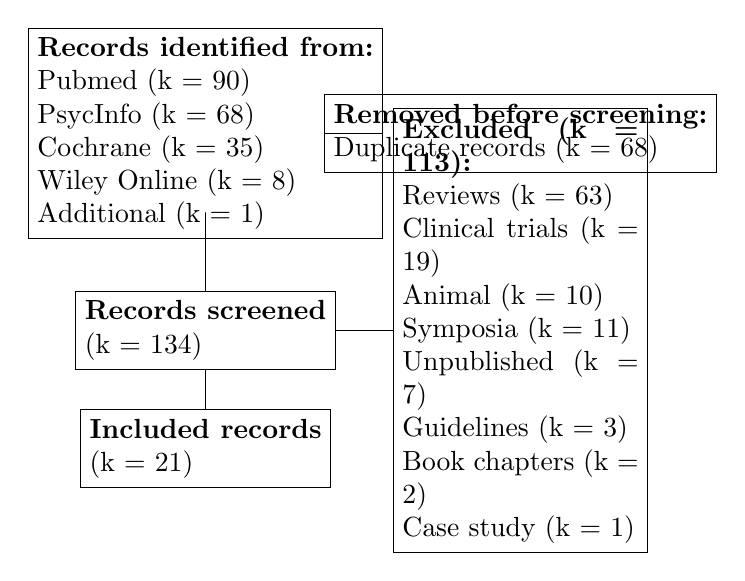
\begin{tikzpicture}[level distance = 40mm,sibling distance = 5mm]
%%%%%%%%%%%%%%%%%%%%%%%%%%%%%%%%%%%%%%%%%%%%
%%%%%%%%%%%%%%% BOXES %%%%%%%%%%%%%%%%%%%%%%%
% LEVEL 1 %%%%%%%%%%%%%%%%%%%%%%%%%%%%%%%%%%%%%%%%%%%ù
\node (1) at (-1,0)[draw]{\pbox{10cm}{
\textbf{Records identified from:}\\
Pubmed (k = 90)\\
PsycInfo (k = 68)\\
Cochrane (k = 35)\\
Wiley Online (k = 8)\\
Additional (k = 1)
}}
%_________________________________________________
child[grow = right]{node[draw]{\pbox{5cm}{
\textbf{Removed before screening:} \\
Duplicate records (k = 68)
}}} ;
% LEVEL 2 %%%%%%%%%%%%%%%%%%%%%%%%%%%%%%%%%%%%%%%%%%%%%%%%
\node (3) at (-1,-2.5) [draw]{\pbox{5cm}{
\textbf{Records screened}\\
(k = 134)
}}
%_______________________________________________
child[grow = right]{node[draw]{\pbox{3cm}{
\textbf{Excluded (k =  113):}\\
Reviews (k = 63)\\
Clinical trials (k = 19)\\
Animal (k = 10)\\
Symposia (k = 11)\\
Unpublished (k = 7)\\
Guidelines (k = 3)\\
Book chapters (k = 2)\\
Case study (k = 1)
}}} ;
% LEVEL 3 %%%%%%%%%%%%%%%%%%%%%%%%%%%%%%%%%%%%%%%%%%%%%%%%%%%%%%%%
\node (4) at (-1,-4) [draw]{\pbox{3cm}{
\textbf{Included records}\\ 
(k = 21) 
}} ;

%%%%%%%%%%%%%%%%%%%%%%%%%%%%%%%%%%%%%%%%%%%%
%%%%%%%%%% ARROWS %%%%%%%%%%%%%%%%%%%%%
%%%%%%%%%%%%%%%%%%%%%%%%%%%%%%%%%%%%%%%%%%%%
\draw (node cs:name = 1,anchor = south)
|- (-1,-1) -| (node cs:name = {3},anchor = north);

\draw (node cs:name = {3},anchor = south)
|- (-1,-3) -| (node cs:name = {4},anchor = north);

\end{tikzpicture}
\caption{Flow chart}
\label{fig:flowchart}
\end{figure}
%-------------
\begin{figure}[t!]
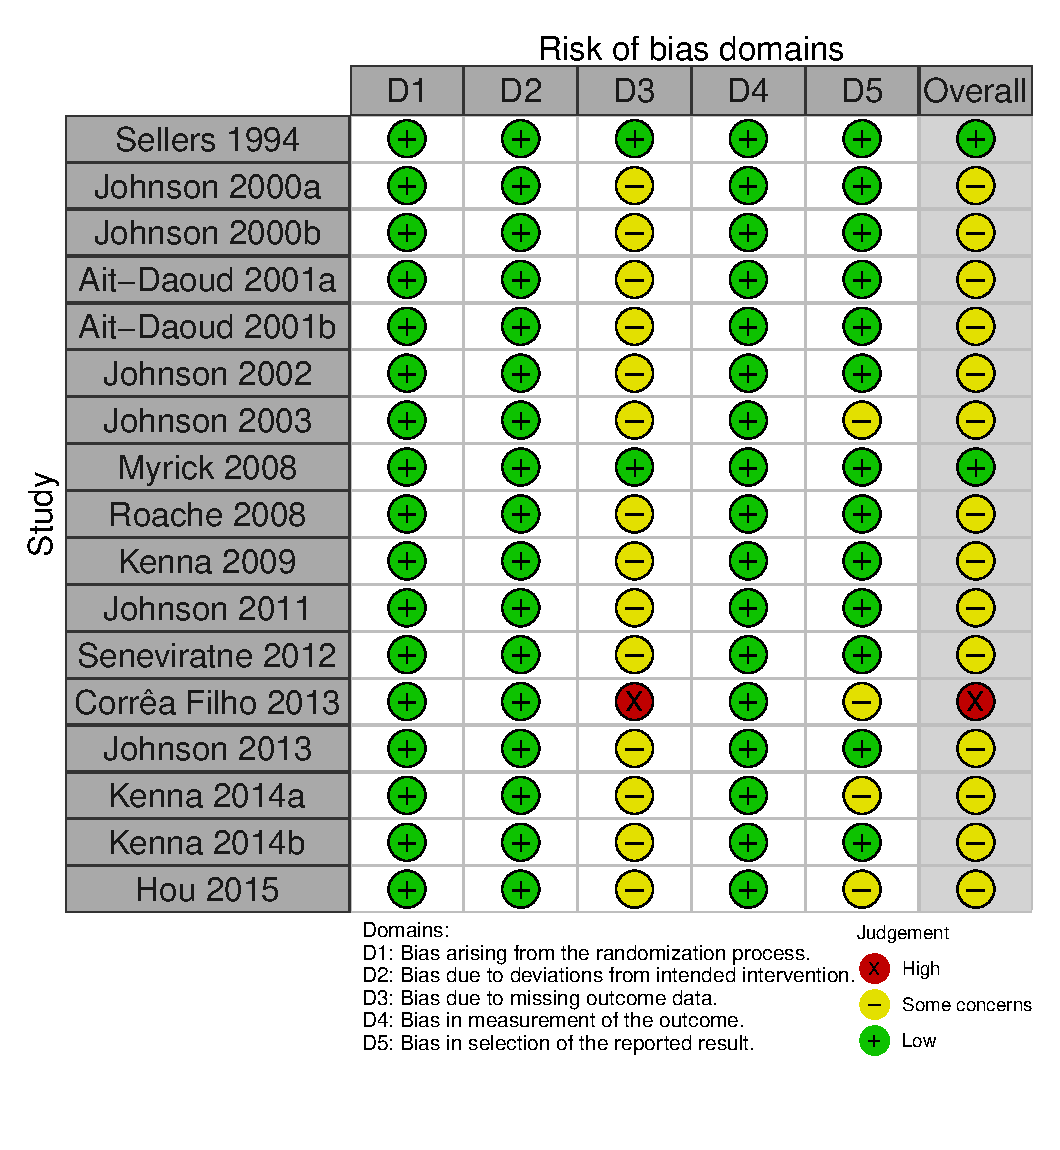
\includegraphics[width=\columnwidth]{pictures/ROB2.eps}
\caption{Risk of bias traffic-light plot (Cochrane Rob2) for the 19 RCT.}
\label{fig:trafficlight}
\end{figure}
%---------------
%---------------------------------------------------------------------------

\begin{table*}[]
\scriptsize
  \centering
   \caption{Newcastle-Ottawa Scale}
  \label{tab:nos}
\begin{tabular}{cccccccccc}
 \hline
 &&&&&&&&&\\
& \pbox{1.7cm}{\textbf{SELECTION}} 
&&&
& \pbox{2cm}{\textbf{COMPARABILITY}}
& \pbox{1.7cm}{\textbf{OUTCOME}}
&&
& \textbf{SCORE}\\

& \pbox{1.7cm}{Representative-\\ness of the \\exposed cohort}
& \pbox{1.7cm}{Selection of \\the non \\exposed \\cohort}	
& \pbox{1.7cm}{Ascertainment\\ of exposure}
& \pbox{1.7cm}{Demonstration that outcome\\ of interest\\ was not\\ present at\\ start of study}

& \pbox{2cm}{Comparability\\ of cohorts on\\ the basis of\\ the design\\ or analysis}

& \pbox{1.7cm}{Assessment\\ of outcome }
& \pbox{1.7cm}{Was\\ follow-up\\ long enough\\ for outcomes\\ to occur}
& \pbox{1.7cm}{Adequacy\\ of follow up \\of cohorts} 
&\\

&&&&&&&&&\\
 \hline
&&&&&&&&&\\
%------------------------------------------------------------
\pbox{3cm}{Kranzler 2003\\ \cite{kranzler_effects_2003}}
&*&*&*&*&*&&*&*&7/9\\
%-----------------
&&&&&&&&&\\
\pbox{3cm}{Dawes 2005a\\ \cite{dawes_prospective_2005}}
&*&*&*&*&N.A.&&*&*&6/7\\
%-----------------
&&&&&&&&&\\
\pbox{3cm}{Dawes 2005b\\ \cite{dawes_reductions_2005}}
&*&*&*&*&N.A.&&*&*&6/7\\
%-----------------------------
&&&&&&&&&\\
 \hline
\end{tabular}
\caption*{N.A.: non applicable (studies without a control group)}
\end{table*}
%---------------------------------------------------------------------------


\end{document}